\documentclass[tikz]{standalone}
\begin{document}
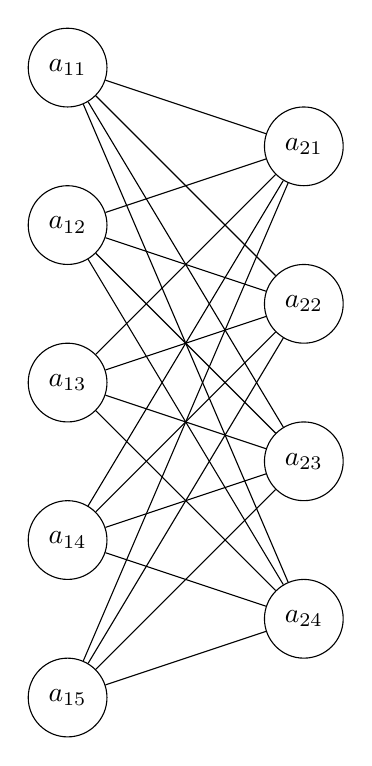
\begin{tikzpicture}
  \tikzstyle{neuron}=[circle, draw, minimum width=1cm];
  \foreach \x in {1,...,5} {
    \node [neuron] (a\x) at (0, -2*\x) {$a_{1\x}$};
  }
  \foreach \y in {1,...,4} {
    \node [neuron] (b\y) at (3, -1-2*\y) {$a_{2\y}$};
  }
  \foreach \x in {1,...,5} {
    \foreach \y in {1,...,4} {
      \draw (a\x) edge (b\y);
    }
  }
\end{tikzpicture}
\end{document}